Diante da visão da IoT propõe-se detectar efeitos colaterais indesejáveis de uma maneira inteligente em um HNS (Figura \ref{fig:hnsworkmodel}), mais especificamente no cenário ``Levar compras'' (seção \ref{sec:cenario}). O cenário ``Levar compras'' foi desenvolvido com o intuito de criar um ambiente no HNS que tivesse efeitos colaterais indesejáveis. Uma vez que há efeitos colaterais indesejáveis, surge a necessidade de se detectar estes efeitos. O método de detecção destes efeitos utilizou meta-classificação com o intuito de gerar um modelo satisfatório para esta detecção (seção \ref{ch:validacao}). Uma vez que o modelo foi validado, este foi implantado no cenário ``Levar compras'' do FIM.

\begin{figure}[!htb] \centering 
  \centering
  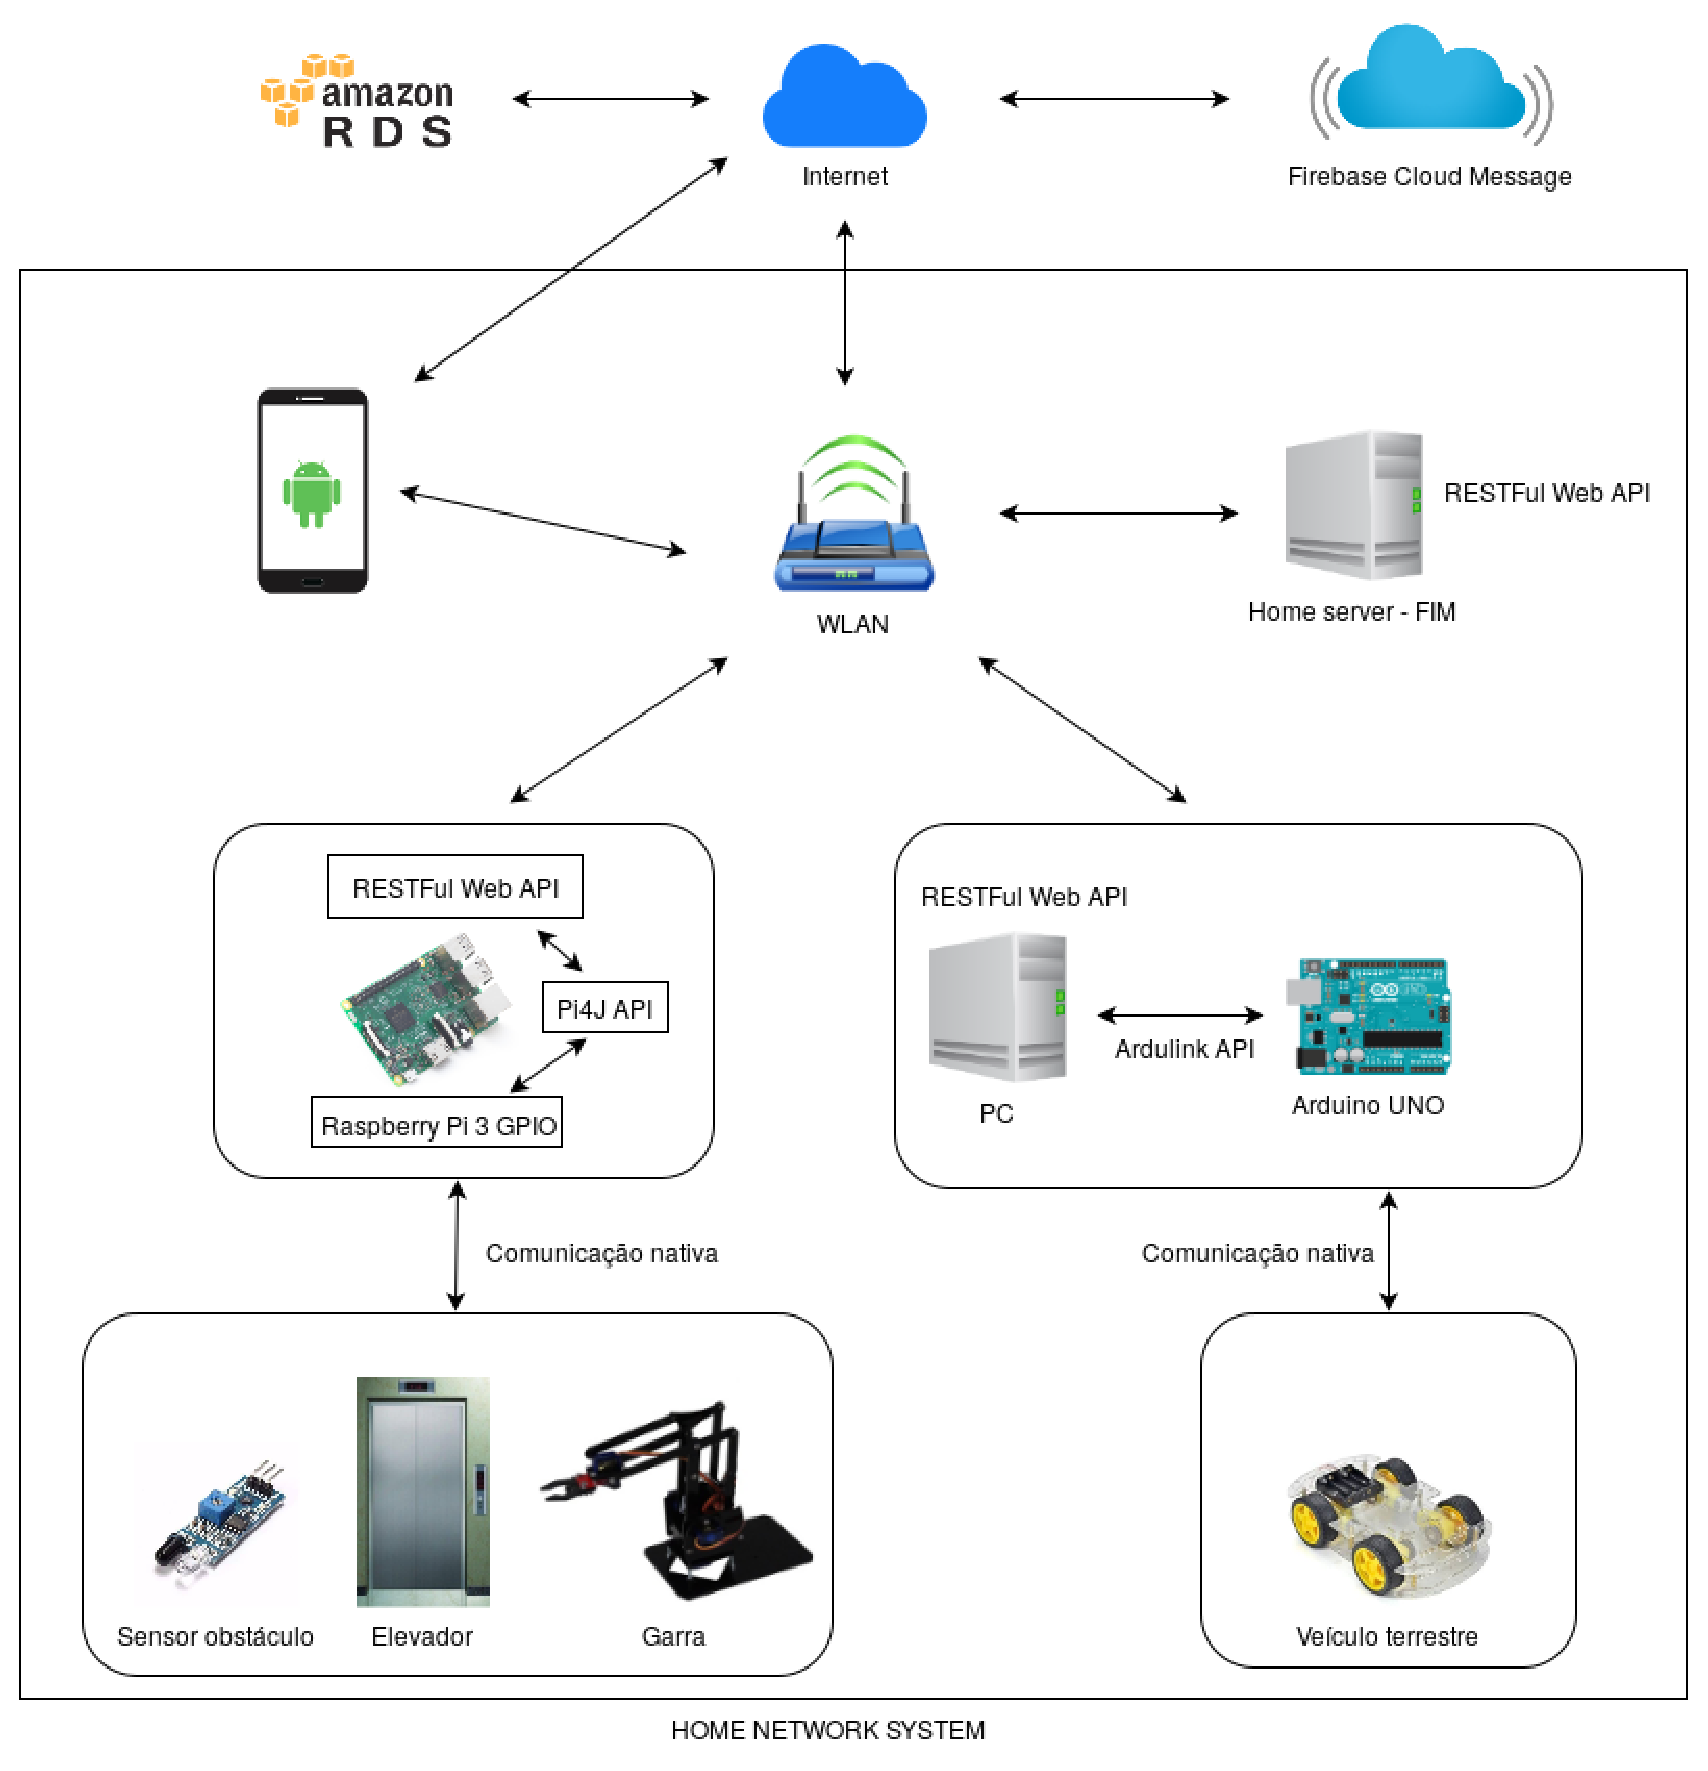
\includegraphics[width=1.0\columnwidth]{cenario} 
  \caption{Modelo do HNS utilizado neste trabalho.} 
  \label{fig:hnsworkmodel}
\end{figure}

\section{Efeitos colaterais indesejáveis no HNS (Cenário Levar compras)}
\label{sec:cenario}
O cenário ``Levar compras'' refere-se a incorporação de efeitos colaterais indesejáveis no HS. Esta funcionalidade é provida através da composição dos serviços do elevador, veículo e garra. O cenário em questão pode ser visualizado na Figura \ref{fig:cenario} e é descrito a seguir.

\begin{enumerate}
\item Um usuário da casa (morador ou visitante), organiza as compras numa cesta (que tem formato expansível) e a coloca sobre o veículo terrestre.
\item O usuário então aciona o serviço ``Levar compras'' (disponibilizado pelo HS) através do seu \textit{smartphone}. O serviço então começa sua execução.
\item O FIM solicita informações de restrições do elevador e veículo terrestre, assim como quais objetos compõem a cesta. Este então verifica se a cesta colocada sobre o carro quebrou alguma restrição do mesmo e se a massa total dos objetos excedem a carga máxima do elevador.
\item Se nenhuma destas restrições foram quebradas o FIM solicita ao veículo terrestre que leve a as compras até as proximidades do elevador.
\item Assim que o veículo chega no seu destino, este envia uma mensagem ao FIM informando de sua chegada.
\item O FIM então requisita o elevador para levar as compras.
\item O elevador agora solicita a garra mecânica que pegue o cesto e coloque-o dentro do elevador.
\item Quando a garra completa a execução do seu serviço, esta avisa ao elevador.
\item Caso não haja nenhuma restrição, como por exemplo, alguma coisa que possa impedir a porta do elevador de fechar, então o elevador inicia o transporte das compras ao seu destino final e manda uma notificação ao HS.
\item HS Captura token referente ao \textit{smartphone} com Android\footnotemark \footnotetext{\url{https://www.android.com/intl/pt-BR_br/}} do usuário da casa. Por fim, o HS solicita ao serviço de notificação \textit{Firebase Cloud Message}\footnotemark \footnotetext{\url{https://firebase.google.com/docs/cloud-messaging/?hl=pt-br}} que envie uma notificação para o usuário da casa, que a recebe no seu \textit{smartphone}. Assim completa-se a execução do serviço ``Levar compras''.
\end{enumerate}
        
\begin{figure}[!htb] \centering 
  \centering
  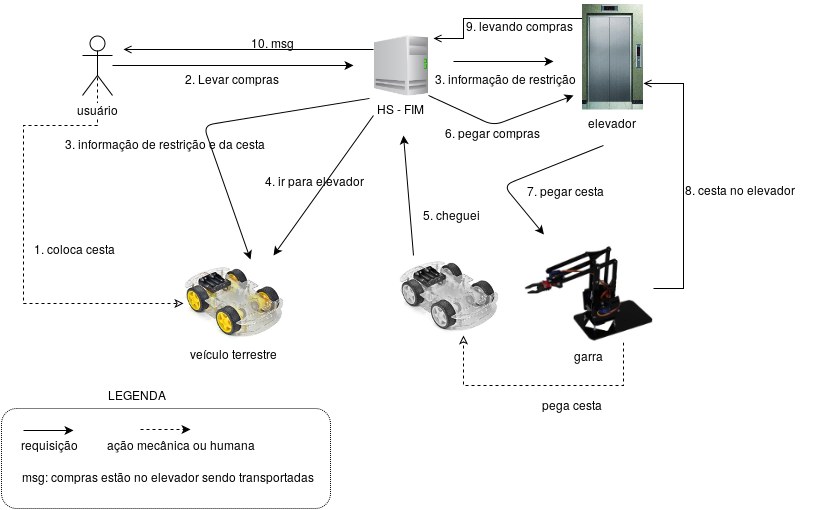
\includegraphics[width=1.0\columnwidth]{cenario_requests} 
  \caption{Cenário Levar compras.} 
  \label{fig:cenario}
\end{figure}

No cenário descrito da Figura \ref{fig:cenario} o elevador não contém motores nem algum outro tipo de sistema elétrico ou mecânico, este é representado por uma caixa de papelão e um sensor de obstáculo acoplado. O veículo terrestre é representado por um programa carregado no Arduino UNO\footnotemark \footnotetext{\url{https://www.arduino.cc/en/Main/ArduinoBoardUno}}, o qual escuta através de sua porta serial mensagens provindas do PC (Figura \ref{fig:cenario}) e as processa simulando as funcionalidades ``Ir para elevador'' e ``cheguei''. Pela mesma porta serial o veículo terrestre encaminha suas mensagens ao PC. Os dispositivos veículo, elevador e garra podem ser visualizados na Figura \ref{fig:cenario_real}.

\begin{figure}[!htb] \centering 
  \centering
  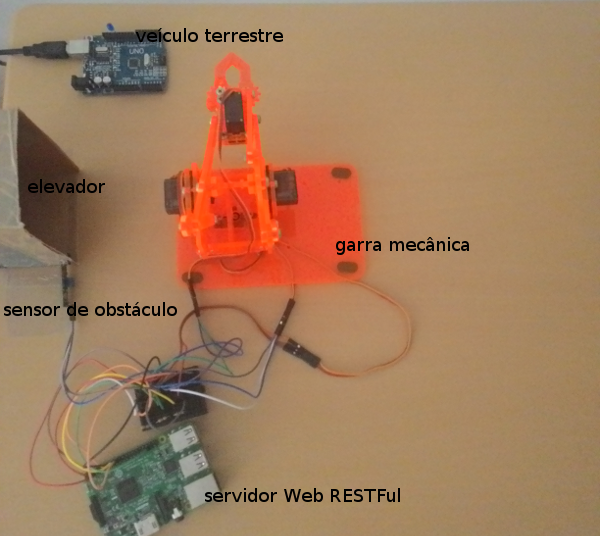
\includegraphics[width=0.8\columnwidth]{cenario_foto_real} 
  \caption{Dispositivos reais do cenário ``Levar compras''.} 
  \label{fig:cenario_real}
\end{figure}

\subsection{Execução do cenário Levar compras}
De acordo com a Figura \ref{fig:cenario} o primeiro passo para inicializar a execução do cenário é colocar a cesta no veículo terrestre. Apesar do veículo ser simulado através de um software embarcado no Arduino, este necessita das informações dos objetos que se deseja transportar. Sendo assim, as informações da cesta são passadas quando o usuário executa o passo 2 (Levar compras). O usuário digita o ``id da cesta'' (no banco de dados) que se deseja transportar e clica em um botão para inicializar o serviço. Todas as cestas são compostas com miniaturas de objetos que normalmente são encontrados em supermercados, exemplos de cestas podem ser visualizados na Figura \ref{fig:exemplos_cesta}. Todos os objetos e cestas estão cadastradas no banco de dados na nuvem (amazon RDS\footnotemark \footnotetext{\url{https://aws.amazon.com/pt/rds/postgresql/}}), o qual foi apresentado na Figura \ref{fig:hnsworkmodel}. A lista de objetos que podem fazer parte de uma cesta é demonstrada na Figura \ref{fig:lista_objetos}, observe que para cada objeto é cadastrado suas características de massa, largura, comprimento, altura e diâmetro.

\begin{figure}[!htb] \centering 
  \centering
  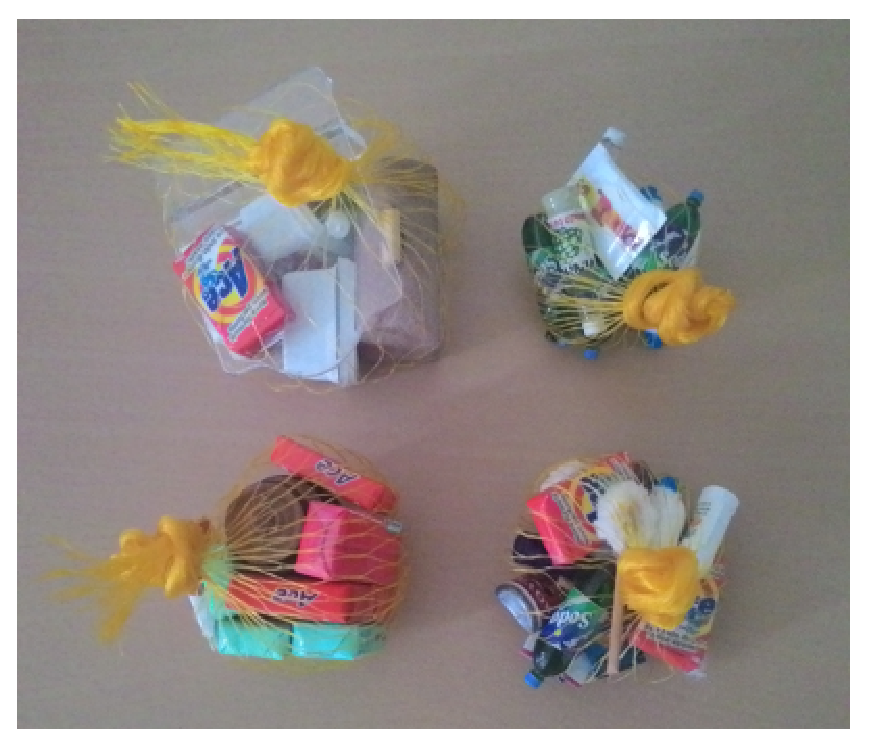
\includegraphics[width=0.8\columnwidth]{experimento/exemplos_cesta} 
  \caption{Exemplo de cestas do cenário ``Levar compras``.} 
  \label{fig:exemplos_cesta}
\end{figure}

\begin{figure}[!htb] \centering 
  \centering
  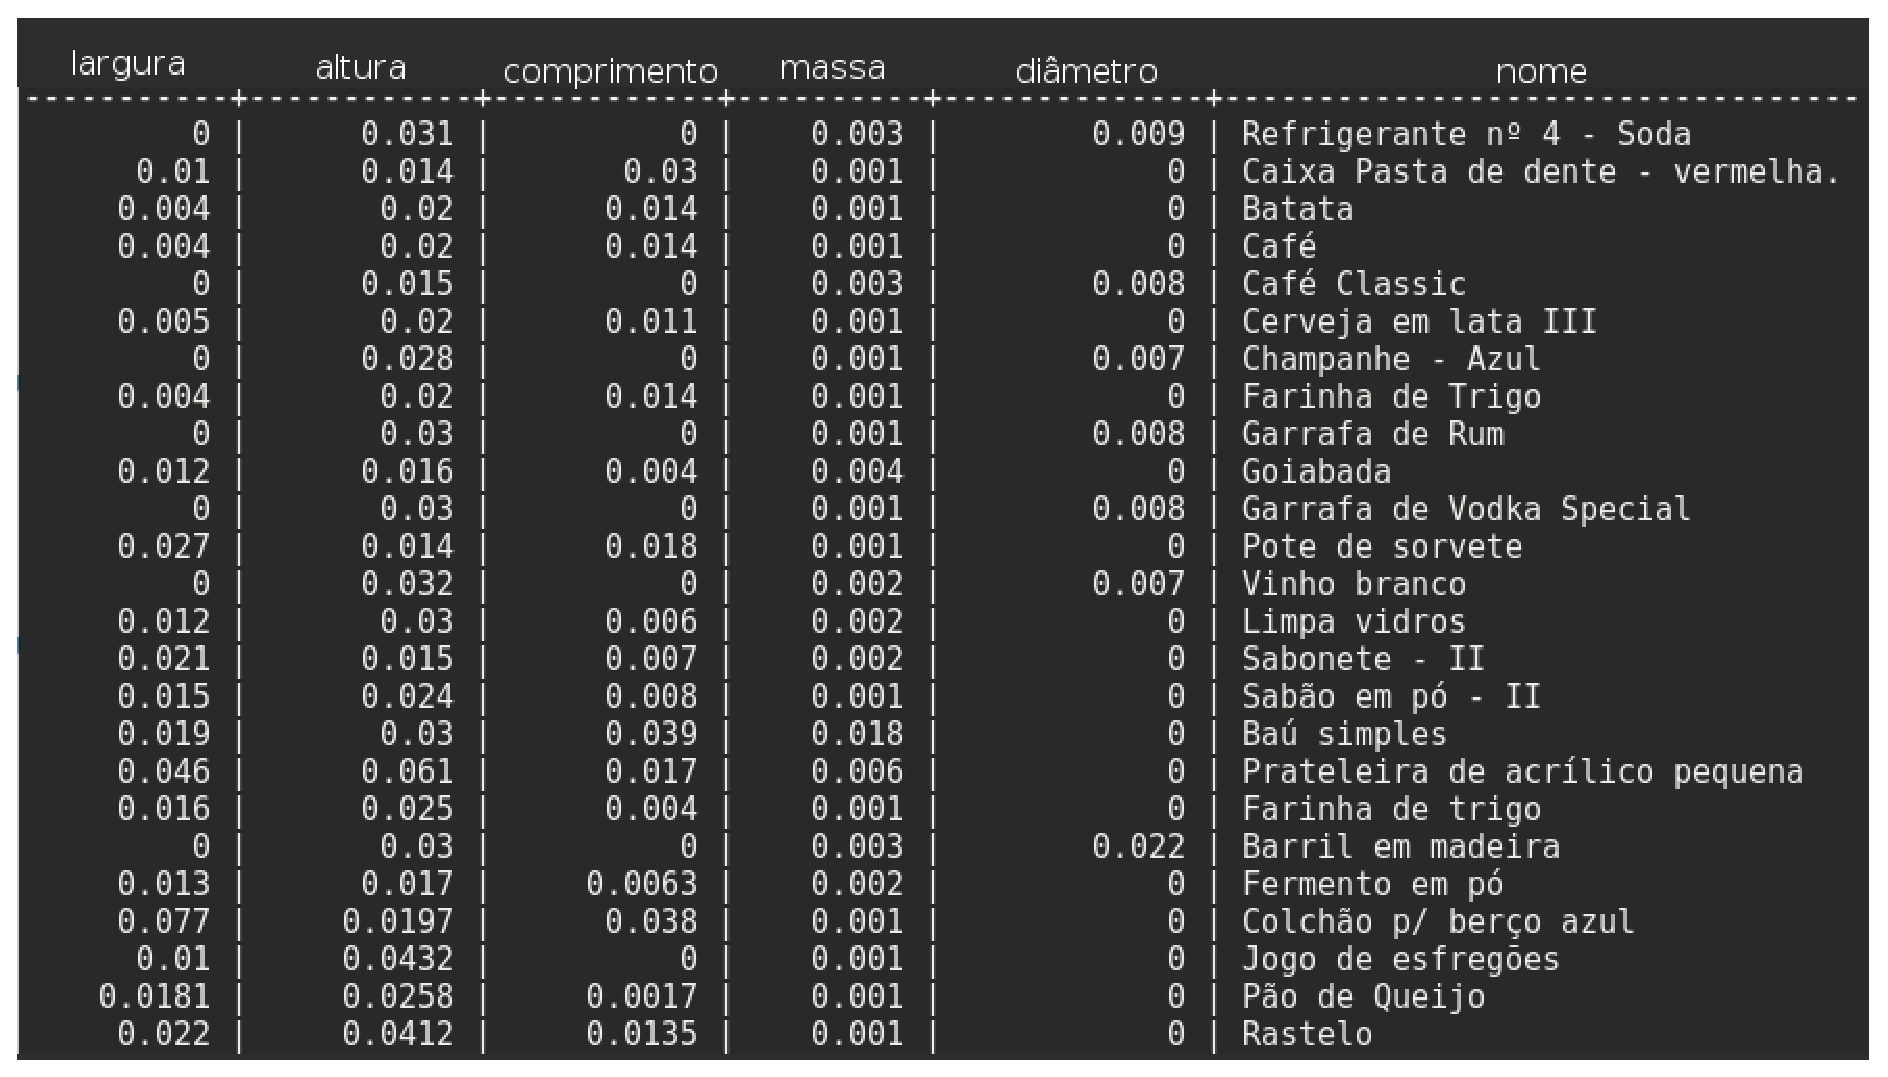
\includegraphics[width=0.8\columnwidth]{experimento/lista_items} 
  \caption{Lista dos objetos que podem ser utilizados para compor uma cesta.} 
  \label{fig:lista_objetos}
\end{figure}

Os próximos passos (3, 4, 5, e 6) do cenário já têm a informação necessária e não necessita de nenhuma intervenção humana. Isto já não acontece com o passo 7 (pegar cesta), pois este necessita de intervenção humana para a garra poder pegar a cesta e continuar a realizar o seu serviço, é preciso posicionar a cesta no lugar correto para a garra prender a cesta, como pode ser visto na Figura \ref{fig:garra_pegando_objeto}. Então, após a garra executar seu serviço esta manda uma mensagem para o elevador e, caso não tenha nada obstruindo a porta do elevador este inicia o transporte da cesta até o local desejado e manda uma mensagem para o FIM. Daí em diante a execução do cenário continua da mesma forma com já explanado.

\begin{figure}[!htb] \centering 
  \centering
  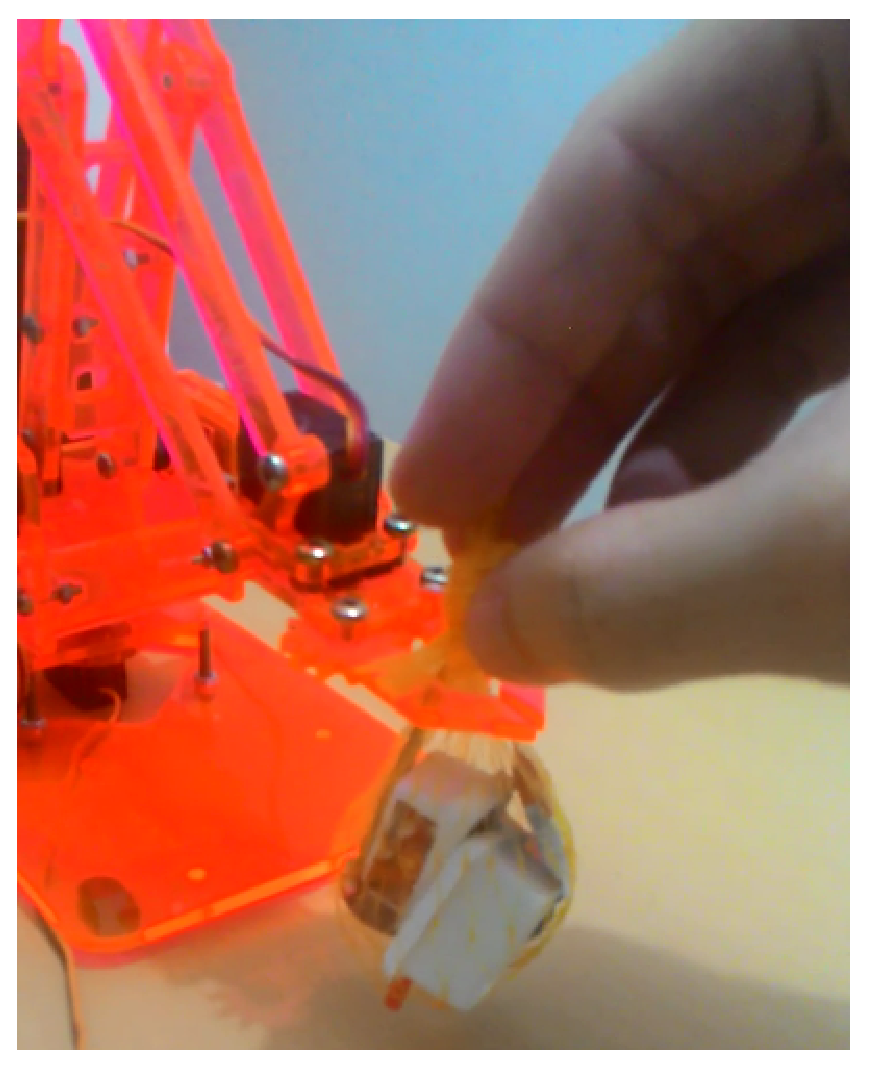
\includegraphics[width=0.8\columnwidth]{experimento/garra_pegando_objeto} 
  \caption{Cesta posicionada no local adequado por um humano, para que a garra possa prender a cesta adequadamente.} 
  \label{fig:garra_pegando_objeto}
\end{figure}

\section{Método de detecção}
\subsection{Geração da massa de dados}
\label{subsec:geracaodados}
A geração da massa de dados para o desenvolvimento do método proposto de detecção ocorreu de forma real. Os dados gerados foram obtidos através da execução do cenário ``Levar compras''. Para a execução deste cenário foram confeccionadas e cadastradas no banco de dados 59 cestas distintas. Antes de registrar as cestas no banco sempre era observado se a cesta cabia dentro do elevador quando colocadas de forma manual, e se também não ultrapassava os limites da porta, o limite de detecção do sensor de obstáculos. Então a cesta só era registrada caso coubesse no elevador e não estivesse em área que pudesse obstruir a porta. Diante das observações da execução do cenário, percebeu-se que as informações das cestas poderiam ser um indicativo ao problema (efeito colateral indesejável) provocado pelo comportamento da garra. Como todas as cestas estavam previamente cadastradas no banco de dados, a estas foram atribuídos valores de ``é efeito colateral'' ou ``não é efeito colateral'', à medida que se observava cada execução do cenário. Desta forma, para construção do modelo (seção \ref{sec:constvalidacao}) que classifique o problema em ``é efeito colateral'' ou ``não é efeito colateral'' utilizou-se as informações das cestas. Vale salientar que a informação da cesta é uma resposta do veículo terrestre referente a requisição ``3'' da Figura \ref{fig:cenario}, ou seja, é uma das informações que os dispositivos e/ou serviços trocam entre si durante a excecução do cenário.

O cenário foi executado 59 vezes, uma para cada cesta, e pode-se observar que em algumas vezes o comportamento da garra provocava um efeito colateral indesejável (seção \ref{sec:featureinteraction}) à funcionalidade ``Levar compras'', pois para todos esses casos se esperava sempre como resultado o elevador levar as compras sem problemas, já que era sabido que as cestas cabiam no elevador e, nenhuma delas feria as restrições de massa do carro nem do elevador. 

A garra durante a execução da sua funcionalidade provocava a locomoção dos objetos. Esta locomoção ocorria em diferentes momentos da execução da funcionalidade: no momento em que a garra pegava o objeto, quando fazia os movimentos (direita, esquerda, cima, baixo, frente trás) ou no momento em que os objetos eram postos no compartimento do elevador. No momento em específico de por os objetos dentro do elevador, além dos objetos as vezes gerarem outras dimensões de cesta, esta também poderia se locomover, devido a natureza dos objetos e da forma como os objetos eram soltos pela garra. Por esse motivo utilizou-se a cesta como informação para construção do modelo.

\subsection{Seleção dos atributos}
\label{sec:selecaodados}
Os dados coletados na etapa de execução do cenário ``Levar compras'', 59 cestas, ainda estão muito brutos. Uma cesta pode conter um objeto, como também pode conter muitos. Supomos que a cesta tenha 10 objetos, então o total de características da cesta seria ``$10 \times 5=50}$'', pois cada objeto possui cinco características. Utilizar as características dos objetos desta forma terá um custo computacional muito elevado. Para diminuir a quantidade de atributos e melhor qualificá-los gerou-se características a partir de todos os atributos dos objetos da cesta: média das alturas, dos comprimentos, das larguras, dos diâmetros e das massas, assim como o total de cada uma dessas medidas, e o total de itens. De ínicio então têm-se a seleção de 11 parâmetros.

Com a seleção prévia desses atributos, constriu-se um arquivo ``arff'', que é o tipo de arquivo padrão utilizado como \textit{dataset} pelo Weka \cite{Hall:2009}. Este \textit{dataset} é composto de 59 instâncias (referente as 59 cestas), cada uma com 11 atributos mais um que identifica a qual classe pertence (``é efeito colateral'' ou ``não é efeito colateral''). Então têm-se 11 atributos númericos e um nominal (a classe a qual a instância pertence).

O próximo passo utilizado nesse processo de seleção de atributos foi o de visualizar estes novos parâmetros par a par, e verificar quais pares parecem melhor separar as classes ``é efeito colateral'' ou ``não é efeito colateral''. A Figura \ref{fig:plotall1} passa a ideia de tal visualização. 

\begin{figure}[!htb] \centering 
  \centering
  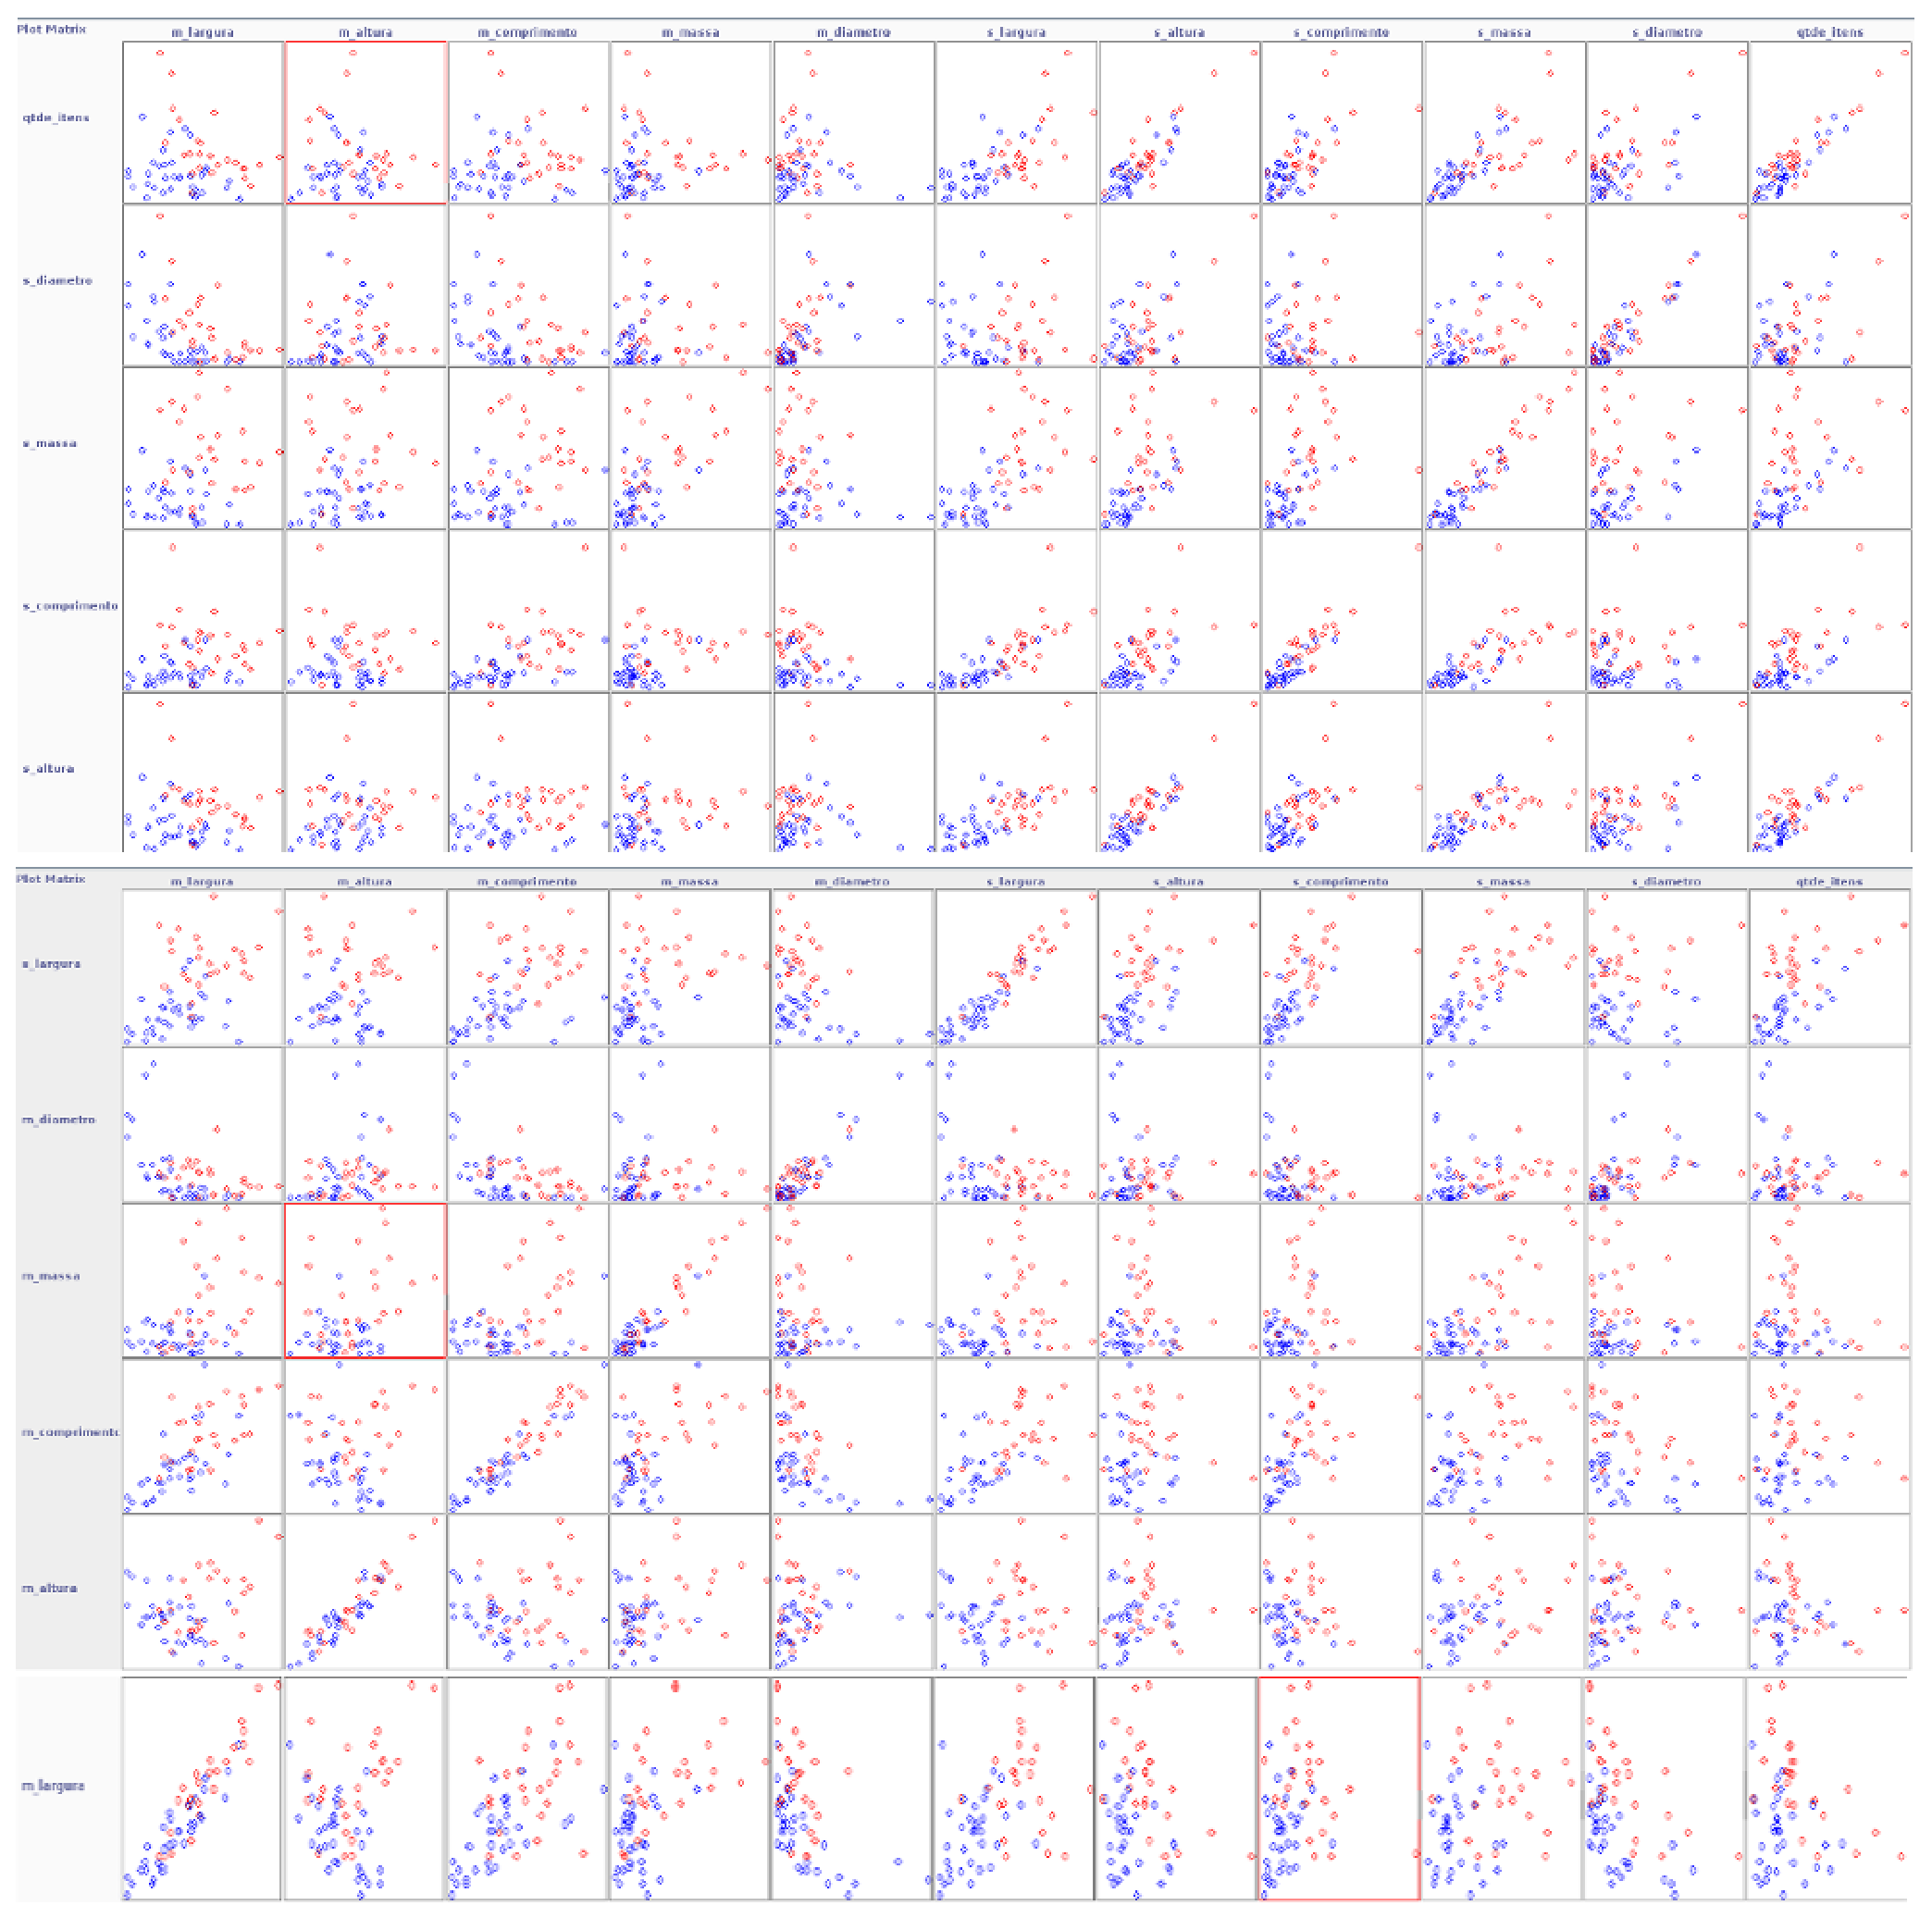
\includegraphics[scale=0.3]{experimento/all_plot} 
  \caption{Plotagem do espaço de \textit{features} par a par do \texit{dataset} de 59 instâncias.} 
  \label{fig:plotall1}
\end{figure}

Dentre essas plotagens foram selecionadas três da Figura \ref{fig:eixos_4_atributos}, as quais aparentam melhor separar as classes, são respectivamente os pares ordenados (somaLargura, somaMassa) - ``sl x sm'', (somaDiâmetro, somaLargura) - ``sd x sl'' e, (médiaAltura, somaLargura) - ``ma x sl''.

\begin{figure}[!htb] \centering 
  \centering
  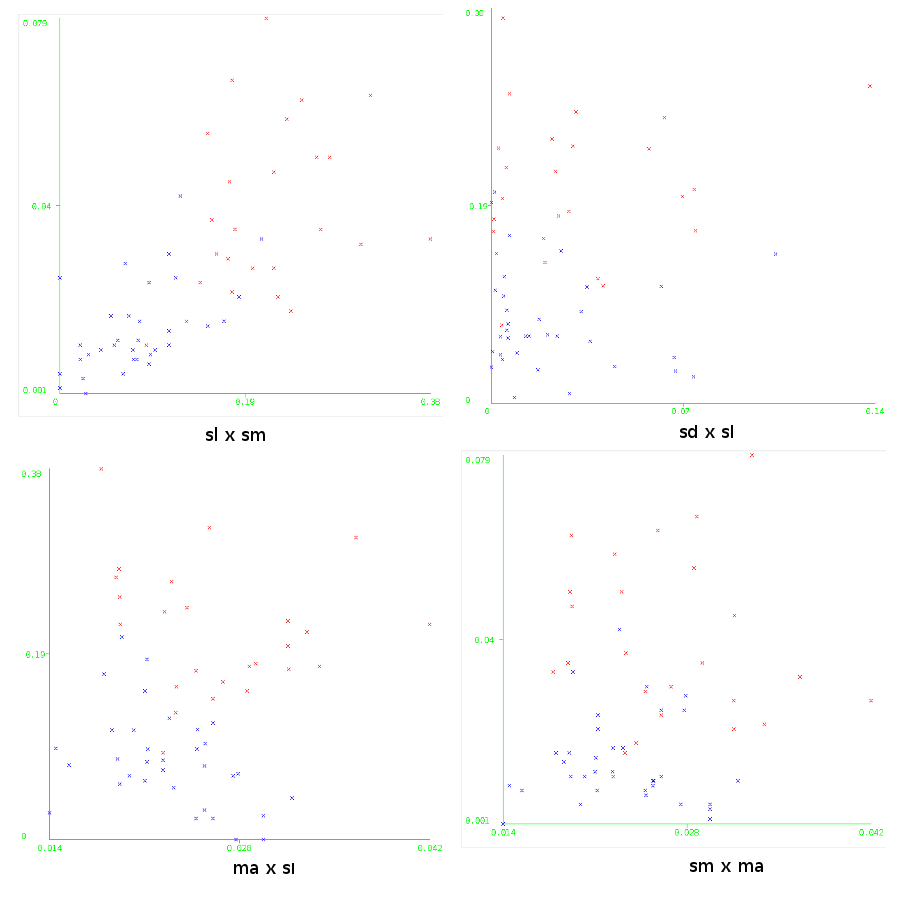
\includegraphics[width=0.8\columnwidth]{experimento/eixos_4_atributos} 
  \caption{Separação das classes entre os atributos (somaLargura, somaMassa) - ``sl x sm'', (somaDiâmetro, somaLargura) - ``sd x sl'' e, (médiaAltura, somaLargura).} 
  \label{fig:eixos_4_atributos}
\end{figure}

Então, nesta fase de seleção dos atributos, estes foram os pares selecionados para construção e validação do modelo (seção \ref{sec:constvalidacao}). Observe que o espaço de \textit{features} foi reduzido a duas características.

\subsection{Meta-classificador DECORATE}
Os parâmetros do DECORATE escolhidos neste trabalho foram semelhantes a um dos testes avaliativos realizados em \cite{Melville:2004}, nos quais comparam \textit{DECORATE} com outros métodos classificatórios, em diferentes tamanhos de dataset e diferentes parâmetros do DECORATE. Para as avaliações neste trabalho o número de iterações é setado em 50, o número máximo de classificadores participantes no \textit{ensemble} é setado em 14, o classificador base utilizado é o J48 e, a quantidade de exemplos artificiais gerados em cada iteração é setado para 100\% (valores setados de 50\% a 100\% não faz variar muito o resultado \cite{Melville:2004}) do tamanho do dataset de treino.

\section{Implantação do método proposto}
\label{sec:implmetprop}
O classificador atua exatamente no momento em que o serviço veículo responde a requisição do FIM na etapa 3 da Figura (\ref{fig:cenario}). Nesta etapa o veículo primeiramente captura o ``id\_cesta'' (banco de dados) passado a ele pelo FIM. Então o veículo utiliza uma funcionalidade do serviço FIM que captura a cesta correspondente ao ``id\_cesta'', transforma-a em um arquivo ``arff'' contendo somente uma instância com os parâmetros correspondentes a ``somaLargura, mediaAltura, classe'', sendo a classe com valor não rotulado, ou seja, não sabe-se a qual classe pertence (``é efeito colateral'' ou ``não é efeito colateral''). O FIM então salva este arquivo e retorna o caminho do arquivo como resposta para o dispositivo veículo. O veículo então responde a requisição 3, sendo um dos dados o caminho do arquivo ``arff'' referente a cesta. Neste momento o FIM utiliza o classificador (uma funcionalidade interna) para predizer se ``é efeito colateral'' ou ``não é efeito colateral'' passando como parâmetro ao classificador o caminho do arquivo ``arff''. Caso o classificador classifique como ``é efeito colateral'' o FIM interrompe o serviço e manda uma mensagem para o usuário informando que ocorreu ``efeito colateral indesejável. Caso contrário o fluxo do cenário (Figura \ref{fig:cenario}) continua e no final da execução o usuário recebe uma mensagem de sucesso.
